\chapter{Sketch It, Make It: Overview}

The primary contribution of this thesis is the set of interaction
techniques implemented in a single design tool called Sketch It, Make
It (SIMI). SIMI is a modeling environment for laser cutter design that
recognizes short sequences of drawn input made with a stylus. Using
only freehand input, SIMI enables a designer to iteratively and
incrementally create precise laser cut models.

I am inspired by the potential of freehand drawing as the basis for
precision modeling for several reasons. Sketching is quick and can be
easily learned. It is simple and modeless: unlike structured editing
software, a designer need not set a pencil's mode to line, circle, or
anything else. I will show that given an appropriate set of
interaction methods, sketched input can provide enough information to
make a precise digital model.

There are several principles that guided SIMI's design and development.

\begin{itemize}
\item \textbf{Democratized design}: Freehand drawing is a skill that
  most people already have. It follows that a tool based on sketch
  based interaction should be usable by a majority of people. For this
  reason I target avocational designers, not professionals. 
\item \textbf{Sketch based}: The user should never feel obliged to set
  down their pen. In the past, many sketch based design tools have
  relied on keyboard input, or used interface widgets that are
  appropriate for mice but are uncomfortable to use with a stylus
  (e.g. hierarchic menus).
\item \textbf{Coherence of interaction techniques is key}: The tool
  presents a set of sketch based interaction techniques that work well
  together. Researchers commonly make toy systems that demonstrate one
  or two novel interaction techniques in isolation (e.g. my own prior
  work on Flow Selection~\cite{johnson-flow-selection}). But a useful
  tool has many individual techniques. The current system implements
  many techniques together to give an example of a way to make them
  work harmoniously.
\item \textbf{Useful and usable}: Last, the system lets people make
  real things in a real domain (namely, laser cut objects). The
  current implementation of the tool is efficient and highly
  responsive. In informal demonstrations, more than one person has
  noted that the system seems more like a commercial product than a
  research system. This is intentional.
\end{itemize}

\section{Rapid Fabrication and Laser Cutting}

Laser cutters are among the more common and affordable fabrication
machines. One can think of a laser cutter as a fast, strong, and
precise automated razor that cuts flat material (paper, wood, plastic,
textiles, etc.). 

% Price information: 
% 2001: 12,900 (ULS 25 watt)
% 2006: 9,995 (ULS 25 watt)
% 2010: 8,500 (ULS 25 watt)
% 2011: 6,850 (ULS 25 watt)
%
%   http://www.rcgroups.com/forums/showthread.php?t=16912 claims that
%   a 25-watt model from Universal Laser systems cost $12,900. Several
%   comments in that thread are in line with that price estimate for
%   home-garage-lab use.
%   http://www.microgeo-usa.com/ProductDetails.asp?ProductCode=universal-laser-VLS2.30
%   currently prices the ULS 25 watt 16x12 unit as costing $6,850.

% http://55-website.com/xo1/ulsinc/english/PDFs/EJ_VL_Article_Reprint.pdf is a press article from 2006 that prices the 25 watt laser at 10,000
\begin{figure}[b] %  figure placement: here, top, bottom, or page
   \centering
   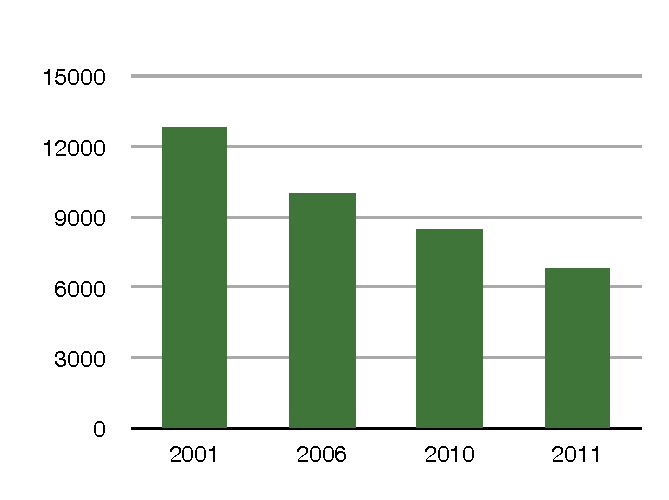
\includegraphics[width=3in]{img/prices.pdf} 
   \caption[Declining laser cutter prices]{Declining prices of Universal Laser Systems 25-Watt 16x12
     inch laser cutter (US Dollars).}
   \label{fig:prices}
\end{figure}


The price of laser cutters is quickly declining, making it possible
that more people have access to them. Figure~\ref{fig:prices} shows
prices for a comparable~25-Watt,~16''x12'' laser cutter model from
Universal Laser Systems (these values were found on hobbyist web
forums). While these data may not be exact, they do show the price of
desktop laser cutting machines has been cut by almost half in the past
ten years. While still out of reach for most people to afford, they
are becoming inexpensive enough for schools and hacker spaces to own.

Laser cut designs are composed of parts cut from solid, flat material
and assembled in various ways: laminated, notched, bolted together,
\textit{etc}. Various materials require different laser speed and
intensity settings to achieve a quality cut. The designe uses a
software application to specify part shapes for laser cutting. The
software outputs vector graphics called a ``cut file'' that defines
these shapes. As most joints have small margins of error, lengths,
angles, and relative position must be specified precisely so that
parts fit together properly.

Tools for designing laser cut objects must allow users to precisely
specify dimensions. Like a physical saw, the laser leaves a gap in its
wake, called a \textit{kerf}, (between 0.2mm and 0.5mm on a 40 watt
cutter). This is an important consideration when designing facets
whose tolerances are small with respect to kerf. A notch joint, for
example, is ineffective if it is 0.1 mm too large or small.


\section{Motivating Scenario: Pictureframe Holder}

\begin{figure}
  \centering
  \begin{subfigure}[b]{0.45\textwidth}
    \centering
    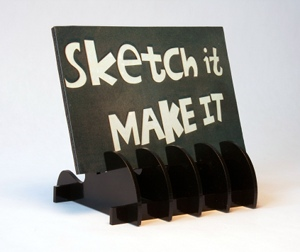
\includegraphics[width=\textwidth]{img/simi-stand-withpic.jpg}
    \caption{} % force the (a) to show up
    \label{fig:example-1}
  \end{subfigure}
  \begin{subfigure}[b]{0.45\textwidth}
    \centering
    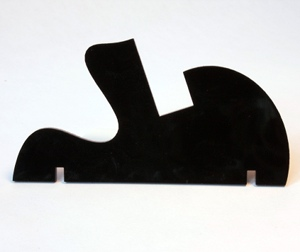
\includegraphics[width=\textwidth]{img/simi-stand-part.jpg}
    \caption{} % force the (b) to show up
    \label{fig:example-2}
  \end{subfigure}
  \caption[Picture Frame Stand]{A picture stand (\subref{fig:example-1})
    drawn and fabricated using SIMI. A single copy of the primary part
    is shown in (\subref{fig:example-2}). }
  \label{fig:simi-example}
\end{figure}


To introduce Sketch It, Make It I will explain how it could be used to
make the picture stand shown in Figure~\ref{fig:simi-example}. This
narrative helps explain the overall user experience while exposing
technical aspects (which are discussed in much greater detail in the
following chapter).

We begin with the idea of a stand with two horizontal rails as a base
and a five-part vertical support structure, joined with notches. Using
SIMI on a tablet device like the Wacom Cintiq shown in
Figure~\ref{fig:simi-intro}, we first draw the rough profile of the
vertical support piece using curved and straight segments. After a
brief period of inactivity, SIMI captures our drawing, straightening
lines, smoothing curves, and connecting curved and straight
segments. We may optionally press a button with our non-dominant hand
to ask SIMI to do this immediately. If we make a mistake (or if we
change our mind), we can recover quickly by scratching out the
unwanted ink, or use an Undo gesture.

After sketching the rough outlines of our two parts, we begin to
refine the design and make it precise.  We square the corners by
drawing right-angle braces (Figure~\ref{fig:motivating}a).  Now as we
adjust the shapes of the two parts by selecting and dragging endpoints
and re-shaping curves, SIMI maintains the right-angle constraints
we've established.
 
Next, we add notches to the two parts for the joints. We draw five
small notches on the base rail. For each notch we draw three lines
inside the outline of the part, and then use the erase gesture to
remove the residual outline segment (Figure~\ref{fig:motivating}b).
Then we indicate that both sides of the notch are to be the same
length: We draw tick marks on each segment, and right-angle braces to
keep the notch perpendicular to the edge of the part. The notches must
have exactly the right dimensions: too wide, the top parts will
wobble; too narrow and they will not fit. We size the notch by
overtracing its segments and entering fixed dimensions
(Figure~\ref{fig:motivating}c).
 
We drag the base part (twice) and the support part (five times) to
SIMI's cut file area to prepare a PDF file for cutting, and then send
it to the laser cutter.  Finally we assemble the cut parts to make the
picture stand in Figure~\ref{fig:simi-example}.

\begin{figure}
  \centering
  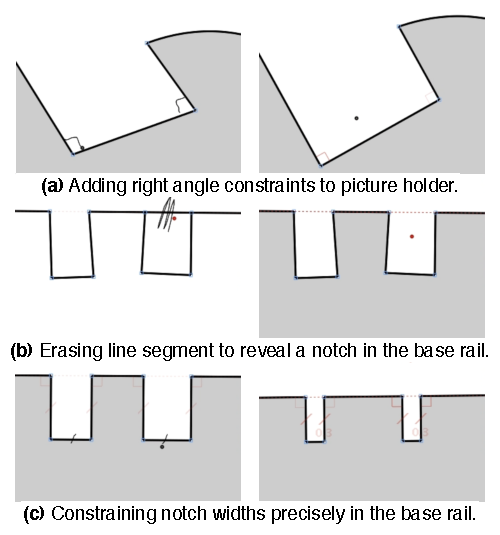
\includegraphics{img/motivating-example.pdf}
  \caption[Interaction steps to a picture frame]{Key steps taken when
    making the picture stand.}
  \label{fig:motivating}
\end{figure}


\section{Technical Challenges Met By SIMI}

The above section describes the user's needs, and how the user
interacts with the system. This section summarizes several categories
of technical challenges the system has to meet in order to support
those user needs. These categories are printed in bold text. Most of
the following topics are described in great detail in the next
chapter.

A fundamental task is \textbf{ink parsing}. While the pen is down, the
system looks for erase gestures. When the user lifts the pen,
non-erase gestures are parsed for corners, and sections of ink are
identified as primitive sub-shapes like lines, curves, and so forth.

SIMI must be able to dependably \textbf{recognize user input}.
Because input is often made quickly and inaccurately, occasional
recognition errors can not be avoided. There are several kinds of
recognized elements. Input might be linework that specifies the
model's geometry. Or, input might be identified as a gesture that
edits the model by removing ink or adding constraints. Last, input
might be as part of a multi-stroke phrase that controls the modeling
environment (e.g. undo/redo, zooming, or panning).

There is one recognizer per recognizable pattern. Each recognizer has
access to the model state, but they do not communicate directly with
each other. Inevitably more than one recognizer will signal a positive
result, so it is necessary for SIMI to \textbf{disambiguate}
contending recognition results. For example, the user may draw two
short strokes that are recognized as both a right angle symbol and a
same-length gesture. To resolve this ambiguity, SIMI uses a series of
tests that involve context (e.g. if the input is correctly positioned
in a corner or not) as well as static precedence rules that defer to
the interpretation that causes the least trouble in the event it is
wrong.


\missingfigure{Need a figure of the overall architecture. Include all
  the parts talked about in this section: ink parsing, recognition,
  disambiguation, data model, and cutfile generation.}

The user's work is stored as a \textbf{data model} consisting of
points, segments (e.g. line, arc), and high-level constraints
(e.g. right angle, same length). SIMI lets the user edit the model to
create, merge, or erase these elements. The \textbf{constraint engine}
is closely associated with the data model. This lets the designer
indicate geometric rules that the system will try to maintains, even
as the user edits the model. SIMI's constraint engine is an iterative,
numerical solver using a relaxation method in the tradition of
Sketchpad~\cite{sutherland-sketchpad}.

When it is time for the user's work to be given to a laser cutter, the
designer asks SIMI to \textbf{generate a cutfile}. This is a 2D vector
graphics file specifying geometry of cutouts. The current
implementation is a rather simplistic ``typewriter'' algorithm---it
uses the bounding box of each cutout, placing one next to the other
from left to right, and moving to the next ``line'' when placing a
piece would extend beyond the material bounds.

\section{Coherent Sketch Based Interaction}

Sketch It, Make It presents a fluid interface for making laser cut
parts. The smooth interaction is made possible by combining many
sketch-based techniques into a set of interaction methods that work
very well together. The fluidity is \textit{not} the result of any one
technique, nor is it simply the result of throwing several existing
methods together.

The interaction techniques offered by SIMI were carefully tuned to
work with one another. Each gesture is as distinct from the others as
possible. This does not completely avoid recognition error but it does
mitigate it because the gestures are not often confused with one
another.

SIMI gives visual feedback when appropriate which helps to resolve
possible conflicts. For example, a selected point will move if a
gesture begins nearby. Without visual feedback that the pen is near
enough, it was easy to inadvertently draw linework when the intention
was to move the point.

The interaction techniques have conservative failure states. The
automatic latching algorithm is a good example. The auto-latcher has
parameters about the distance between points and relative angle of
segments. These parameters were intentionally set to err on the side
of not latching segments together, because the consequences of
latching inappropriately are worse than not latching when the user
wanted. To recover from a missed latch opportunity, SIMI provides a
very simple latching gesture.

SIMI's interaction differs from standard design tools and other sketch
based modeling prototypes in several ways.

\subsection{``The mode problem''}

A traditional design tool like Adobe Illustrator is built around the
concept of input modes such as \textit{select}, \textit{draw line}, or
\textit{fill color}. Users activate modes by selecting a menu option,
clicking an onscreen widget, or pressing a keyboard button. The
program interprets user input in terms of the active tool. Sometimes
users are unaware of which mode the program is in, or are unsure how
to change to the desired mode. Managing modes often introduces
cognitive load by forcing users to think about the tool rather than
their work. This is called ``the mode
problem''~\cite{tesler-mode-problem}.

SIMI's interaction lacks persistent mode. The user can always draw on
any part of the drawing canvas, and the input's meaning is determined
via recognition: an input stroke might be an erasure scribble or a
right angle symbol or a straight line that completes a shape. There is
no `erase mode', no `right angle mode', and no 'draw line mode'. Some
operations, such as flow selection, include transient mode changes
where the meaning of user input is interpreted differently based on
recent interaction. For this reason it is not strictly correct to
label SIMI's interaction as \textit{modeless}.

\subsection{Conversational Interface}

One property that characterizes sketch based systems is \textit{when}
recognition is performed (see
Section~\ref{sec:recognition-when}). Many sketch based design tools
operate in batch mode, where a substantual amount of raw ink is
analyzed at the same time. The rationalle for this approach is that
recognizers have more data (unrecognized ink) to work with and can use
statistical methods to generate the most likely interpretations for
the entire sketch.

SIMI takes a different approach involving short sequences of input
followed by recognition that fix the meaning of input by graphically
representing results. Because the meaning of onscreen elements are
known, the next round of recognition can use that knowledge to provide
unambiguous contextual clues. As the user and system take turns on
such a regular basis, I call this a \textit{conversational
  interface}. The user and the system constantly check each other's
states to ensure that meaning is shared.

\section{Recognition Architecture}

SIMI's recognizers operate at three different times. First,
\textit{Dynamic} recognizers (like Erase) operate while the pen is
down. A second class of recognizers are invoked when the pen is
lifted. If there are positive results from these \textit{Pen Up}
recognizers, action is taken immediately. An example of this kind is
latching. The third kind of recognizer is triggered after a period of
inactivity (currently 1.5 seconds). The user may optionally press a
button with their non-dominant hand to invoke these recognizers on
demand. These recognizers include those that establish constraints
like right angles, or create linework like circles and splines. This
last type is called \textit{Delayed} because it does not happen
immediately after the pen lifts.

\begin{figure}[p]
  \centering
  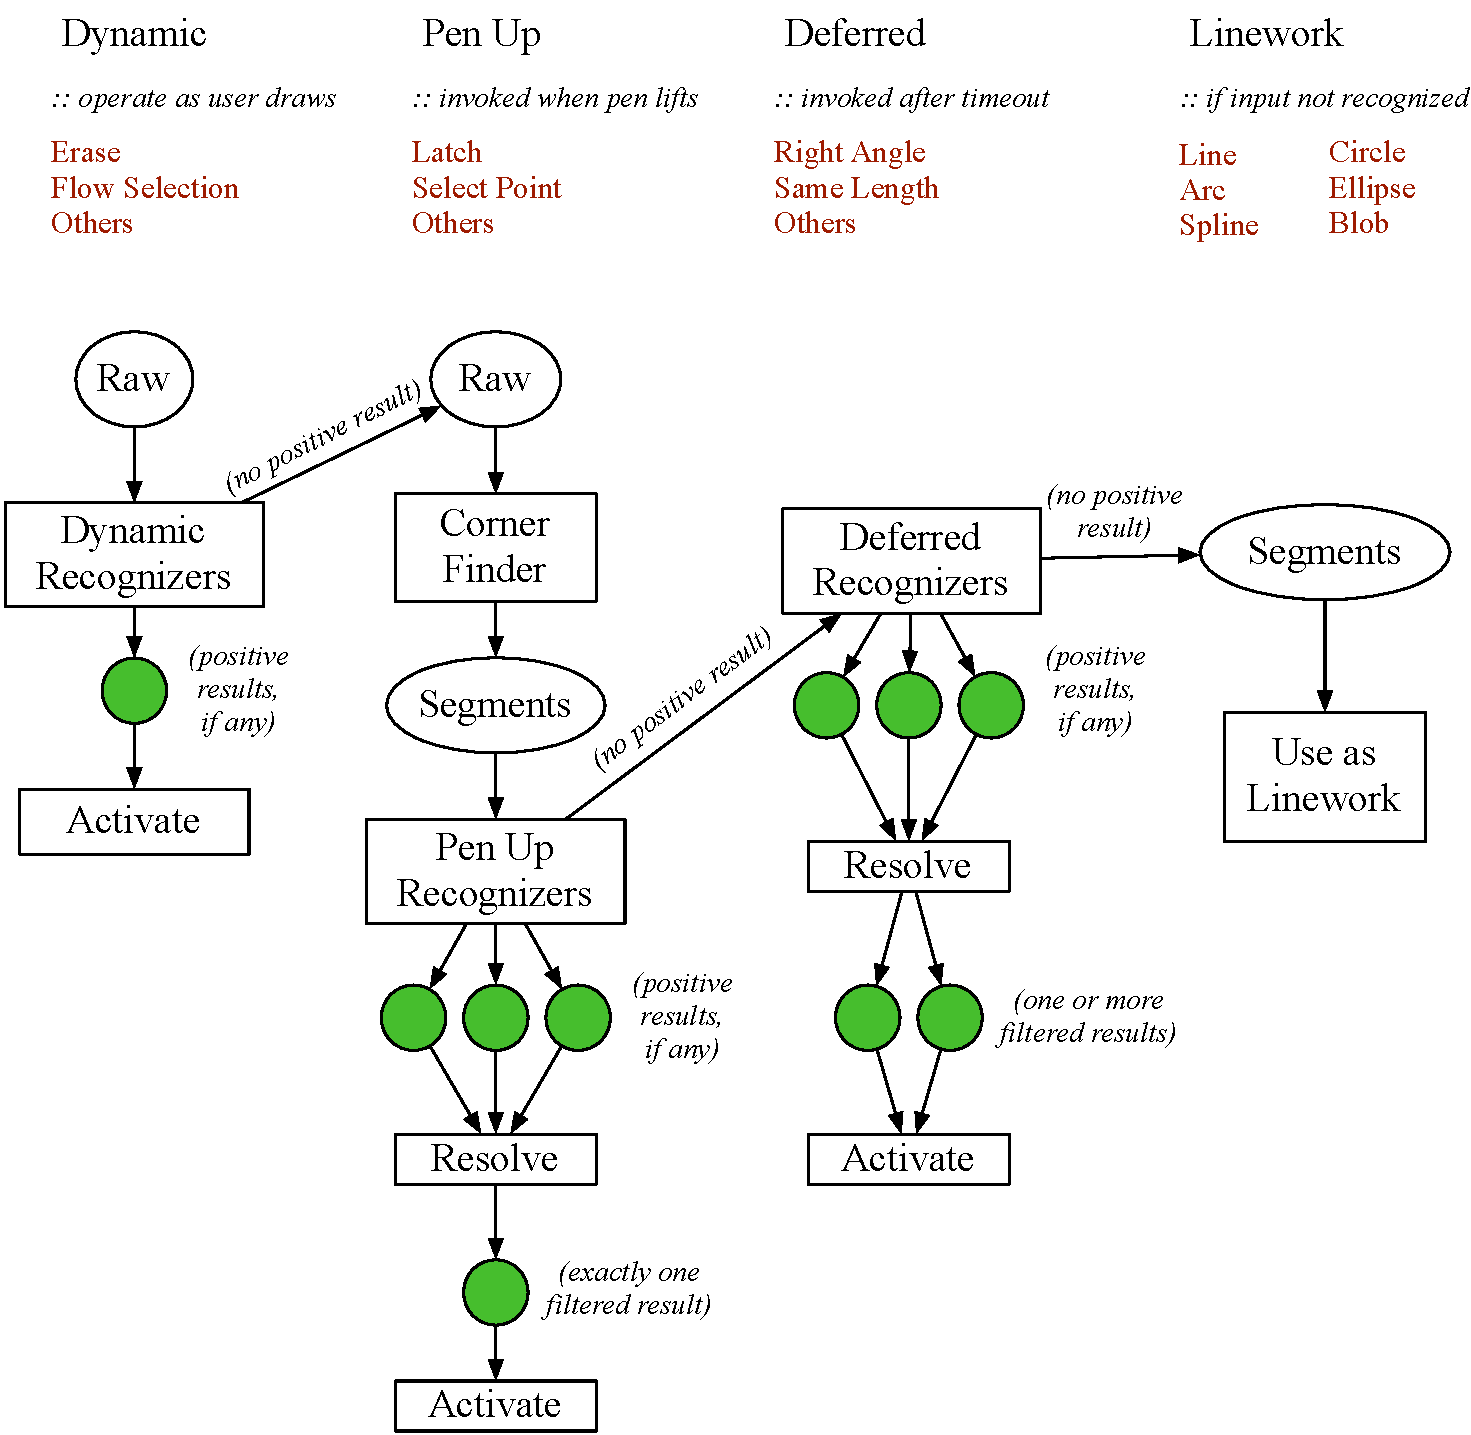
\includegraphics[width=\linewidth]{img/recognition-arch-full.pdf}
  \caption[SIMI Recognition Architecture]{SIMI's recognition
    architecture includes three types of recognizers based on when
    they are invoked. Colored circles indicate positive results.}
  \label{fig:recog-arch}
\end{figure}


Each recognizer class addresses a different need. Dynamic recognizers
allow the user to make gestures that must be recognized as they are
made, when timing is very important. Pen Up recognizers allow the user
to make distinct gestures that are acted on immediately, eliminating
lag and making the interface seem much more responsive. The Pen Up
recognizers are reserved for common actions that are unlikely to
interrupt the user when their associated actions are taken. By their
nature, both Dynamic and Pen Up recognizers must work on single stroke
gestures. Last, the Delayed recognizers may work on one ore more
strokes, and typically have related actions that might distract the
user if they were invoked right away. The overall recognition
architecture is illustrated in Figure~\ref{fig:recog-arch}.

\subsection{Dynamic Recognizers}

Dynamic recognizers use raw pen data that is generated as the user
draws. They are invoked after each new pen movement event, which
typically happen at a rate of once per 15--20 milliseconds. They must
execute very efficiently in order to avoid causing the interface to
seem unresponsive. If the user interface is redrawn at 60 Hz, each
frame must be drawn in less than 16 ms. Therefore it is very important
that all dynamic recognizers execute in much less than this time
period in order to give the graphics subsystem time to draw the
screen.

When a dynamic recognizer finds a positive result, all other Dynamic
recognizers are temporarily turned off, and the associated ink stroke
will not be passed on to the Pen Up recognizers. For example, if the
scribble recognizer determines that the user is erasing, it displays a
visual indication that it recognizers the erasure, and when the user
lifts the pen, it will attempt to erase something. Further, the
Dynamic recognizer might change how the current ink stroke is drawn.

\subsection{Pen Up Recognizers}

If no Dynamic reconizer claimed an ink stroke, it is processed by the
Pen Up recognizers when the user lifts the stylus. The first step is
to parse the raw ink to identify corners and segments. The
implementation details of SIMI's corner finder are given in
Section~\ref{sec:corner-finder}. The Ink Parser supplies a set of
segments, which may be any of the following types: Dots, Lines,
Elliptical Arcs, Splines, Circles, Ellipses, or Blobs (a spline that
starts and ends at a common point).

Pen Up recognizers operate on this set of new segments. Each
recognizer operates independently of the others. They test if segments
comprising the most recent pen stroke match a pattern. It is possible
for several recognizers to positively identify their gesture, but only
one such gesture is valid. If any positive results are found, a
subsequent process resolves conflicts.

The conflicts are mediated in two ways. First, sometimes a gesture
makes more sense than others in context. A context checker will report
how well a gesture matches the current drawing state with a Yes, No,
or Maybe. If only one contending gesture receives a `Yes' vote, the
other interpretations are discarded. Second, if the context checker
can not resolve the problem, then a static rule list is used. This
list ranks each recognizer type, and the interpretation that is
highest on the list is accepted (the rest are rejected).  

The order of this rule list important. Recognizers that edit the model
are lower on the list than recognizers whose effects can be
ignored. For example, a Latch gesture edits the model, while the
gesture to display the Pan/Zoom widget has only a temporary
response. If the wrong interpretation is made, SIMI will err on the
side of the inconsequential or easily recoverable.

If a positive result is found, it is activated without delay. This
means that the action (defined by the gesture) is applied (which is
defined by the context of the gesture). The related action for a Latch
gesture will combine points and possibly destroy and create segments,
which edits the model and causes the graphical representation to
change.

Last, any ink associated with a positive result is removed from the
model and will not be available to the delayed recognizers.

\subsection{Delayed Recognizers}

Delayed recognizers follow a similar process to Pen Up
recognizers. The delayed recognizers are automatically invoked after
the user has not interacted with the system for a short period
(currently 1.5 seconds). The user may optionally speed invocation by
pressing a button with their non-dominant hand.

By this point, any ink that was positively recognized by a Dynamic or
Pen Up recognizer is not available. Every time the pen is lifted, the
ink is processed in the Pen Up recognition step. Any segments that are
not recognized by the Pen Up step are placed in a set of segments for
the Delayed recognizers. This means Delayed recognizers may operate on
segments made in one, two, or (potentially) many more strokes.

Like in the previous recognition step, each Delayed recognizer
operates independently of the others and may produce a positive
result. \textit{Unlike} the previous step, it is possible that several
results are valid, as long as they are composed of different
strokes. This makes it possible, for example, to issue two Right Angle
gestures and a Same Length command in the same batch, all of which can
be recognized. If two potential results involve some of the same
segments, SIMI eploys the same resolution process from the Pen Up
recognizer step.

When conflicts are resolved, there may be zero, one, or more positive
results. The positive results are activated in no particular
order. This could theoretically cause problems (for example if one
action renders another action nonsensical), but this situation has not
been relevant in the current system.

Any segments that are not associated with positive recognizer results
are interpreted as geometry. This is how the user creates linework
that define laser cut parts. This geometry is then included in the
model with definite identities, which are used in later recognition
processes.

\section{Model: Geometry, Constraints, Cutouts}

\missingfigure{Figure showing the relationship between points,
  segments, low-level constraints, and user constraints.}

%% Data structures are simple: we have points and low-level
%% constraints. List all the low-level constraints and give an example of
%% the anatomy of one, especially how it measures error and how it
%% `knows' how to offer advice to correct that error.

%% Next talk about the higher-level user constraints: a user constraint
%% for right angle is implemented with several low-level constraints. 

%% Now for the iterative, numeric solving algorithm. While explaining how
%% it works, can justify the randomness by showing graphs of total error
%% when the solver did not use much randomness.

%% Explain how the solver relates to the rest of the tool: in a separate
%% thread, sending out signals when it is done or after taking a step (to
%% redraw), and how it is capable of being paused when the user is doing
%% something. This makes the system responsive at all times.


